\documentclass{article}
\author{Andrea Casalino}
\title{How to use Fast QHull}

\RequirePackage[margin=2cm]{geometry}
\geometry{left=2cm,right=2cm,marginparwidth=6.8cm,marginparsep=1.5cm,top=1.5cm,bottom=1.5cm,footskip=2\baselineskip}

\usepackage[T1]{fontenc}
\usepackage[utf8]{inputenc}
\usepackage[default]{lato}
\usepackage{graphicx,color, import}
\usepackage{amssymb, amsmath}
%\usepackage{hyperref}
\usepackage{url}

\begin{document}
\maketitle

\newpage
\section{What is a convex hull?}

The Convex hull of a shape \footnote{The term shape will refer in this document to a generic collection of points in the space. It can be either a compact or a non compact set like for example a set of disconnected vertices.} is the minimum convex volume entirely containing that shape. At this point it is important to define the concept of convexity.
The generic convex shape  $\mathcal{S} =  \lbrace S_1, \cdots, S_N  \rbrace$, is a set of points for which it holds that:
\begin{eqnarray}
\mathcal{S} \mathit{\,is\,convex} & \Rightarrow & \forall S_{A,B} \in \mathcal{S} \wedge \forall r\in[0,1] 
\\
& \Rightarrow & S_A + r \cdot (S_B - S_A) = S(r) \in \mathcal{S}
\end{eqnarray}
i.e. the segment connecting the generic pair of points $S_A, S_B \in \mathcal{S}$, is entirely contained in $\mathcal{S}$. Examples of convex and non convex shapes are reported in Figure \ref{fig:convexity}.
Clearly, the convex hull of a convex object it's the object itself. On the opposite, when dealing with any other kind of shapes, the computation of the convex hull is non trivial to perform. Examples of convex hulls wrapping non convex shapes are reported in Figure 
\ref{fig:convex_hull}.

\begin{figure}
	\centering
\def\svgwidth{0.95 \columnwidth}
\import{./image/}{convexity.pdf_tex} 
	\caption{Examples of a convex shape (left) and a non convex one (right). The segment connecting any pair of points within the shape, it's entirely contained in the shape itself. This is not true for the non convex example on the right.}
	\label{fig:convexity}
\end{figure} 

\begin{figure}
	\centering
\def\svgwidth{0.95 \columnwidth}
\import{./image/}{convex_hull.pdf_tex} 
	\caption{Examples of convex hulls.}
	\label{fig:convex_hull}
\end{figure} 

\section{Convex hull representation: meshes}

In case of 3 dimensional objects, the convex hull is represented by a set of triangular facets, forming a convex mesh. Each facet in the mesh is characterized by the positions of the three vertices delimiting that facet. Since the vertices are shared by the facets,
an efficient representation of a mesh consists of a bipartite set $ \langle \mathcal{V} , \mathcal{I}  \rangle$. $\mathcal{V} =  \lbrace V_1, \cdots, V_N  \rbrace$ defines the coordinates of the vertices pertaining to the mesh, while $\mathcal{I}$ are the so called incidences. The $j^{th}$ element $I_j \in \mathcal{I}$, is a tuple $I_j  = \langle V^j_a, V^j_b, V^j_c \rangle$ specifying the vertices delimiting the $j^{th}$ facet.
Figure \ref{fig:mesh} reports example of mesh representation. Notice that the above representation is able to describe both convex and non-convex meshes. However, in case of convex hull, the resulting mesh will be always convex.


\begin{figure}
\begin{tabular}{cc}
\begin{minipage}[t]{0.35\textwidth}
\def\svgwidth{ \columnwidth}
\import{./image/}{mesh_a.pdf_tex} 
\end{minipage} 
&
\begin{minipage}[t]{0.65\textwidth}
\def\svgwidth{ \columnwidth}
\import{./image/}{mesh_b.pdf_tex} 
\end{minipage} 
\\ 
\begin{minipage}[t]{0.35\textwidth}
\begin{eqnarray}
\mathcal{I} = \lbrace & \langle V_1, V_2, V_3 \rangle & \nonumber\\
& \langle V_1, V_3, V_4 \rangle & \nonumber\\
& \langle V_1, V_5, V_4 \rangle & \nonumber\\
& \langle V_1, V_2, V_5 \rangle & \nonumber\\
& \langle V_2, V_3, V_4 \rangle & \nonumber\\
& \langle V_2, V_4, V_5 \rangle &
\rbrace
\end{eqnarray}
\end{minipage} 
&
\begin{minipage}[t]{0.65\textwidth}
\begin{eqnarray}
\mathcal{I} = \lbrace & \langle V_A, V_B, V_G \rangle & \nonumber\\
& \langle V_B, V_C, V_G \rangle & \nonumber\\
& \langle V_C, V_D, V_G \rangle & \nonumber\\
& \langle V_D, V_E, V_G \rangle & \nonumber\\
& \langle V_E, V_F, V_G \rangle & \nonumber\\
& \langle V_F, V_A, V_G \rangle & 
\rbrace
\end{eqnarray}
\end{minipage} 
\end{tabular}
\caption{Examples of mesh representation. On the left a simple convex object and it's incidences, while on the right a non convex shape with the incidences of some of their facets..}
\label{fig:mesh}
\end{figure} 

\section{Convex hull determination}

FastQHull was conceived to compute the convex hull of a shape whose geometry is described by the coordinates of a point cloud $\mathcal{C} =  \lbrace C_1, \cdots, C_L  \rbrace$. If you are interested in determining the convex hull of a solid object, described for example by a (non convex) mesh, pass as $\mathcal{C}$ the set of vertices pertaining to that solid. Clearly, the resulting convex hull $ \lbrace \mathcal{V}_{CH} , \mathcal{I}_{CH}  \rbrace$ will be such that $\mathcal{V}_{CH} \subseteq \mathcal{C}$ or in other words, the vertices of the convex hull are a subset of the initial point cloud.
The convex hull computation is subdivided into two main steps, described in Sections \ref{sec:step_1} and \ref{sec:step_2}.

\subsection{Phase 1}
\label{sec:step_1}

The algorithm starts by defining an initial tetrahedron that will be then iteratively expanded till converging to the convex hull.
The 4 vertices $ \lbrace V_1,V_2,V_3,V_4  \rbrace$ of the initial tetrahedron are found as described in the following.
\\
$V_1$ is assumed equal to \footnote{$<,>$ stands for the dot product: $<a,b>= a_x \cdot b_x + a_y \cdot b_y + a_z \cdot b_z $}
\begin{eqnarray}
V_1 = argmax_{C_i} \lbrace <\hat{x} , C_i>\rbrace
\end{eqnarray}
with $\hat{x}$ that is the x axis versor, i.e. $\hat{x} = \begin{bmatrix} 1 & 0 & 0 \end{bmatrix}$. Essentially, $V_1$ is identified as the point in the cloud having the maximum value for the $x$ coordinate.
$V_2$ is computed as:
\begin{eqnarray}
V_2 = argmax_{C_i} \lbrace <C_i - V_1,  C_i - V_1> \rbrace
\end{eqnarray}
i.e. the point in the cloud maximising the Euclidean distance w.r.t. $V_1$.
$V_3$ is then computed as:
\begin{eqnarray}
V_3 = argmax_{C_i} \lbrace dist(C_i, \overline{V_{12}}) \rbrace
\end{eqnarray}
where $dist(C_i, \overline{V_{12}})$ stands for the distance between $C_i$ and the line passing between $V_1$ and $V_2$ (see \url{https://en.wikipedia.org/wiki/Distance_from_a_point_to_a_line}). 
Finally, $V_4$ is assumed as:
\begin{eqnarray}
V_4 = argmax_{C_i} \lbrace dist(C_i, \overline{V_{123}})  \rbrace
\end{eqnarray}
where $dist(C_i, \overline{V_{12}})$ stands for the distance between $C_i$ and the plane identified by $V_1$,$V_2$ and $V_3$ (see \url{https://en.wikipedia.org/wiki/Distance_from_a_point_to_a_plane}). 
Figure \ref{fig:tetraedro} summarizes the above steps.
The volume $A$ of the tetrahedron can be computed by considering a triple product (\url{https://en.wikipedia.org/wiki/Triple_product}) \footnote{The operator $\wedge$ indicates the cross product of the two vectors: $c = a \wedge b = \begin{bmatrix} c_x = a_y \cdot b_z - a_z \cdot b_y  & c_y = a_z \cdot b_x - a_x \cdot b_z & c_z = a_x \cdot b_y - a_y \cdot b_x \end{bmatrix}$}
\begin{eqnarray}
A = <V_3 - V_4 ,  (V_2 - V_4) \wedge (V_1 - V_4) >
\end{eqnarray}
In case $A$ results to be close to 0 (or at least 0), it means that the cloud $\mathcal{C}$ is entirely contained in a single plane or a line. In such degenerate cases, the convex hull computations cannot be performed and the procedure is interrupted.

\begin{figure}
	\centering
\def\svgwidth{0.95 \columnwidth}
\import{./image/}{tetraedron.pdf_tex} 
	\caption{Steps involved in the determination of the initial tetrahedron. }
	\label{fig:tetraedro}
\end{figure} 



\subsection{Phase 2}
\label{sec:step_2}


\begin{figure}
	\centering
\def\svgwidth{0.25 \columnwidth}
\import{./image/}{facet_distance.pdf_tex} 
	\caption{Computation of $d$. }
	\label{fig:facet_dist}
\end{figure}

The initial tetrahedron is iteratively updated. At the generic step $k$, the intermediate result $ \lbrace \mathcal{V}_{CH} , \mathcal{I}_{CH}  \rbrace _ {k}$ must be evaluated. The distance $D_j$ of the farthest point from the $j^{th}$ facet in $ \lbrace \mathcal{V}_{CH} , \mathcal{I}_{CH}  \rbrace _ {k}$ is defined as follows:
\begin{eqnarray}
D_j = max_{C_i} \lbrace d(C_i, j)  \rbrace \\
d(C_i, j) = min ( 0 ,\langle C_i - V_a^j , n^j \rangle )
\end{eqnarray}
where $n^j$ is the outer normal versor of the $j^{th}$ facet, refer also to Figure \ref{fig:facet_dist}. The facet having the maximum $D^{*}$ is searched in the mesh $ \lbrace \mathcal{V}_{CH} , \mathcal{I}_{CH}  \rbrace _ {k}$ and the corresponding farthest point $C^{*} \in \mathcal{C}$ is considered. A facet $j$ is said to be visible from $C^{*}$ when it holds that $d(C^{*}, j) > 0$.
The update of the mesh consists in deleting the set of facets visible from the farthest point $C^{*}$, with the aim of replacing them with a cone of new facets. The process is described in Figure \ref{fig:update}.
\\
The algorithm stops when reaching a situation for which $D^{*}$ is equal to 0. Indeed, in such a case all the points in the cloud are already wrapped and the convex hull is computed.

\begin{figure}
	\centering
\def\svgwidth{0.95 \columnwidth}
\import{./image/}{hull_update.pdf_tex} 
	\caption{Convex hull update from step $k$ to $k+1$. The set of visible facets (the blue ones on the left) is replaced with a cone of new facets (visible on the right). }
	\label{fig:update}
\end{figure} 


\section{Accelerating the algorithm using a thread pool}

The computation of the farthest point of a facet (Figure \ref{fig:facet_dist}) can be significantly time consuming when considering clouds $\mathcal{C}$ made of thousands of points. In such cases, the farthest point search can be speed up by considering a thread pool strategy.
Indeed, the computation of the farthest points for the elements in the cone of new facets, Fig. \ref{fig:update}, are parallely dispatched to a pool of thread.
\\
This parallel strategy is convenient only when dealing with clouds made of many vertices, while performance are comparable to the serial standard version when dealing with small-medium size clouds, refer to Figure \ref{fig:times}.

\begin{figure}
\begin{tabular}{cc}
\begin{minipage}[t]{0.5\textwidth}
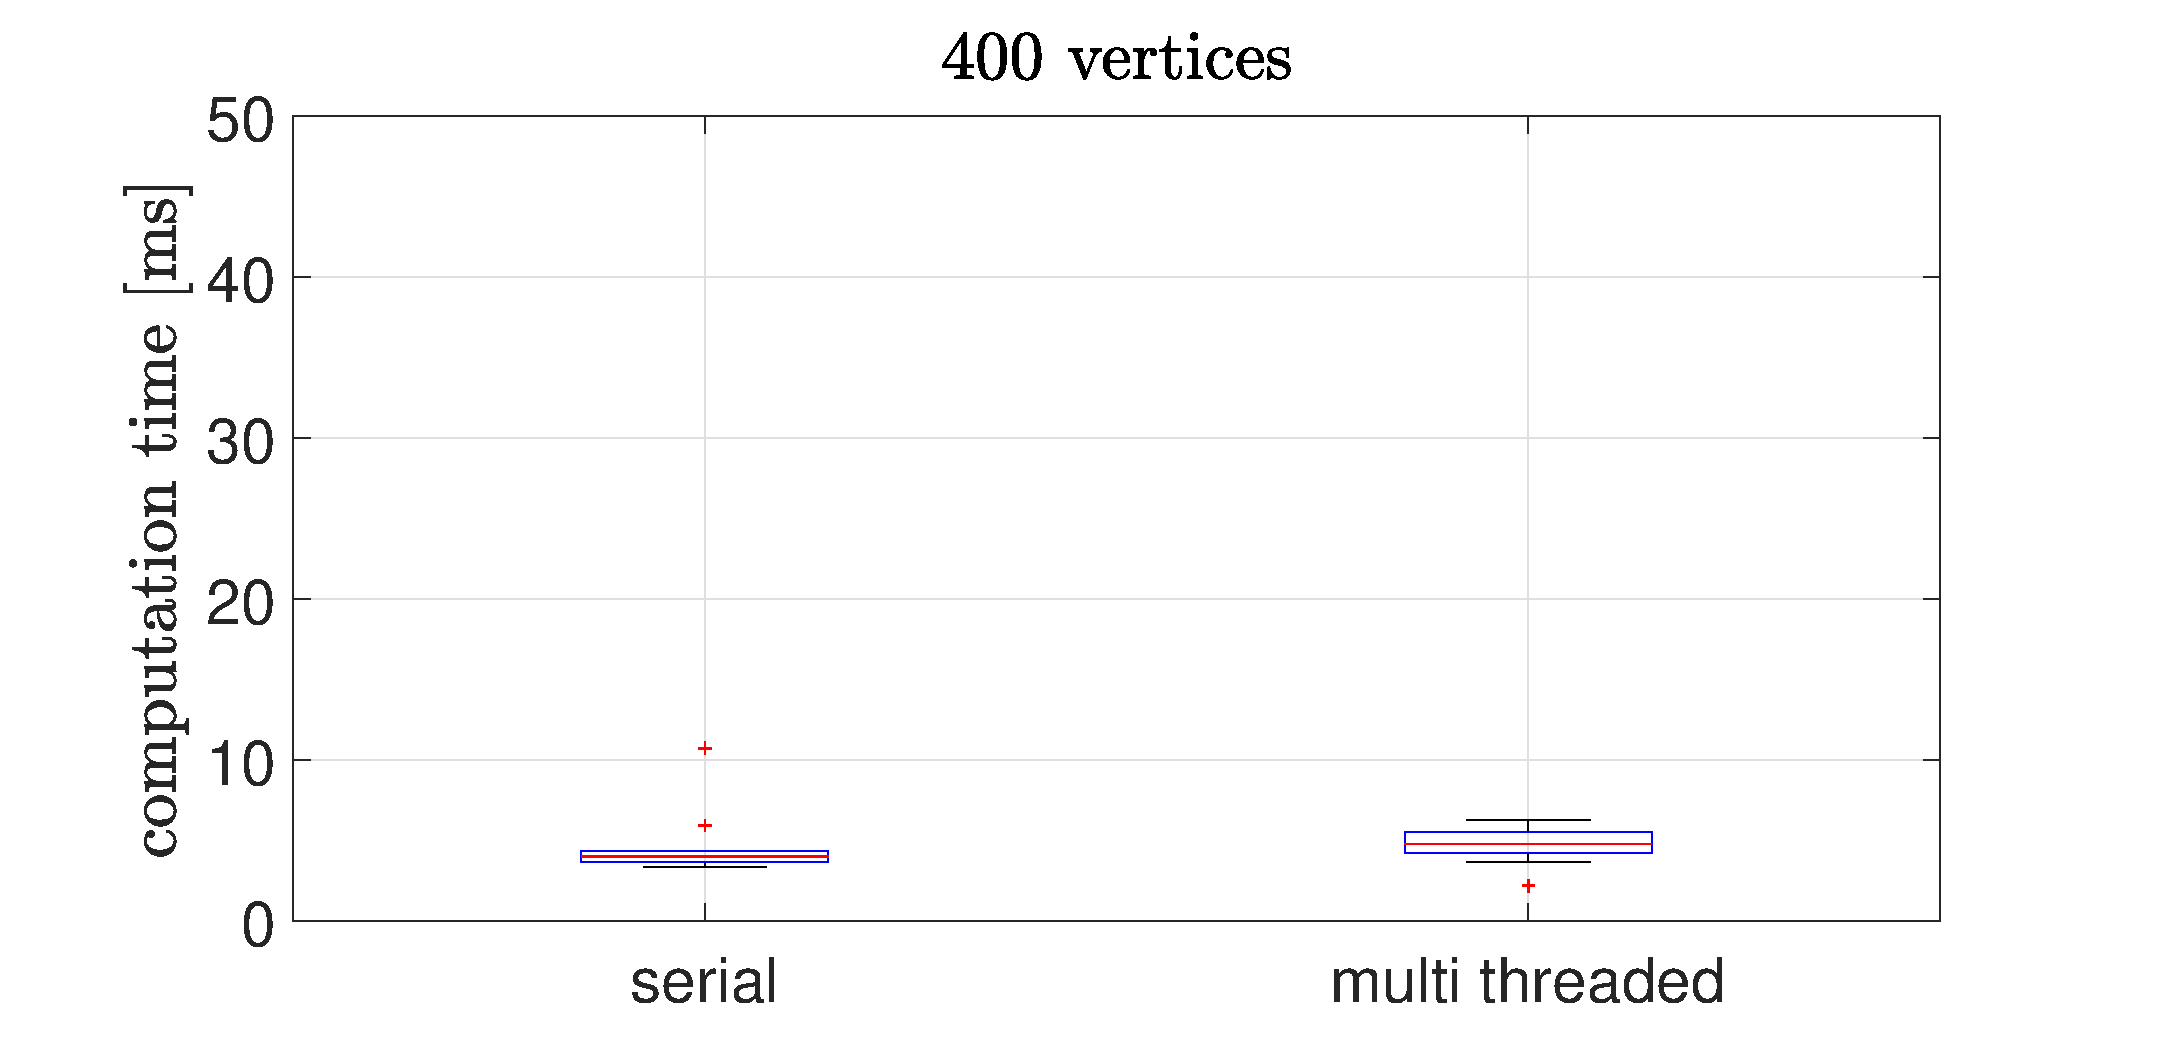
\includegraphics[width = 0.99 \columnwidth]{./image/400_vertex_time.eps}
\end{minipage} 
&
\begin{minipage}[t]{0.5\textwidth}
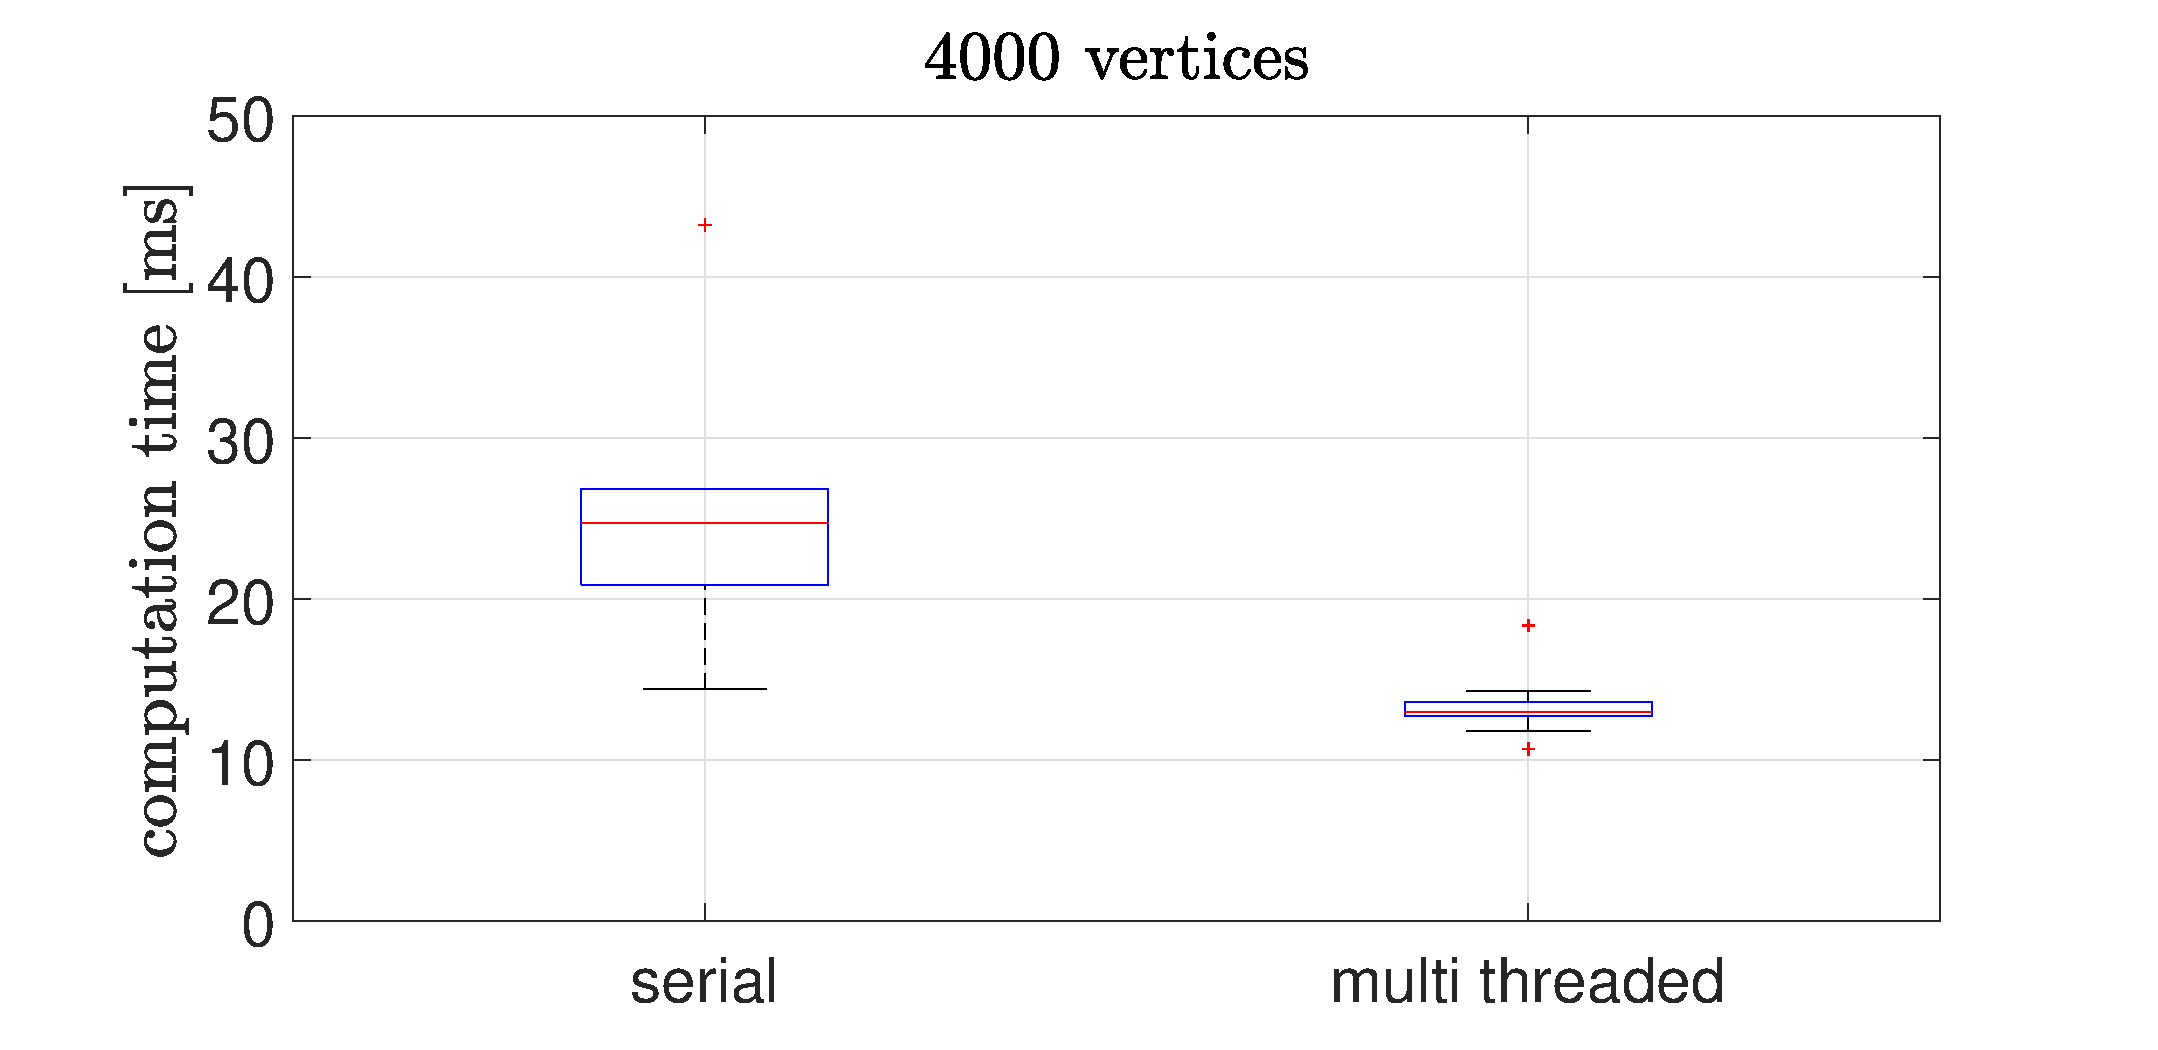
\includegraphics[width = 0.99 \columnwidth]{./image/4000_vertex_time.eps}
\end{minipage} 
\end{tabular}
\caption{Statistics of the time required for computing the convex hull: in the left considering 20 sampled clouds made of 400 vertices, while on the right considering considering to sample clouds made of 4000 vertices. The multi threaded strategy seems to have significant better performance when having many points in the cloud. }
\label{fig:times}
\end{figure} 

 
\end{document}